\chapter{Virittävät puut}

Virittävä puu on kokoelma
verkon kaaria,
joka kytkee kaikki
verkon solmut toisiinsa.
Kuten puut yleensä,
virittävä puu on yhtenäinen ja syklitön.
Usein on kiinnostavaa etsiä
verkon pienin virittävä puu (\textit{minimum spanning tree}),
jonka kaarten painojen summa on mahdollisimman pieni.

Tämä luku esittelee kaksi algoritmia
verkon pienimmän virittävän puun etsimiseen.
Molemmat algoritmit valitsevat puuhun
kaaria ahneesti niin, että joka vaiheessa
puuhun tulee mukaan mahdollisimman kevyt kaari.
Osoittautuu, että pienimmän virittävän puun
tapauksessa ahneet valinnat johtavat
optimaaliseen lopputulokseen.

\section{Kruskalin algoritmi}

Kruskalin algoritmi aloittaa pienimmän
virittävän
puun rakentamisen tilanteesta,
jossa puussa ei ole yhtään kaaria.
Sitten algoritmi alkaa lisätä
puuhun kaaria järjestyksessä
kevyimmästä raskaimpaan.
Algoritmi lisää kaaren mukaan puuhun,
jos sen lisääminen ei muodosta sykliä.

Kruskalin algoritmi pitää yllä
tietoa verkon komponenteista.
Aluksi jokainen solmu on omassa
komponentissaan,
ja komponentit yhdistyvät pikkuhiljaa
algoritmin aikana puuhun tulevista kaarista.
Lopulta kaikki solmut ovat samassa
komponentissa, jolloin pienin virittävä puu on valmis.

\subsubsection{Toiminta}

\begin{samepage}
Tarkastellaan Kruskalin algoritmin toimintaa
seuraavassa verkossa:
\begin{center}
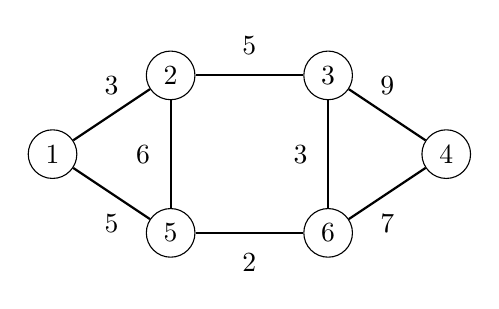
\begin{tikzpicture}
\node[draw, circle] (1) at (1.5,2) {$1$};
\node[draw, circle] (2) at (3,3) {$2$};
\node[draw, circle] (3) at (5,3) {$3$};
\node[draw, circle] (4) at (6.5,2) {$4$};
\node[draw, circle] (5) at (3,1) {$5$};
\node[draw, circle] (6) at (5,1) {$6$};
\path[draw,thick,-] (1) -- node[font=\small,label=above:3] {} (2);
\path[draw,thick,-] (2) -- node[font=\small,label=above:5] {} (3);
\path[draw,thick,-] (3) -- node[font=\small,label=above:9] {} (4);
\path[draw,thick,-] (1) -- node[font=\small,label=below:5] {} (5);
\path[draw,thick,-] (5) -- node[font=\small,label=below:2] {} (6);
\path[draw,thick,-] (6) -- node[font=\small,label=below:7] {} (4);
\path[draw,thick,-] (2) -- node[font=\small,label=left:6] {} (5);
\path[draw,thick,-] (3) -- node[font=\small,label=left:3] {} (6);
\end{tikzpicture}
\end{center}
\end{samepage}
\newpage

Algoritmin ensimmäinen vaihe on
järjestää verkon kaaret niiden painon mukaan.
Tuloksena on seuraava lista:

\begin{tabular}{ll}
\\
kaari & paino \\
\hline
5--6 & 2 \\
1--2 & 3 \\
3--6 & 3 \\
1--5 & 5 \\
2--3 & 5 \\
2--5 & 6 \\
4--6 & 7 \\
3--4 & 9 \\
\\
\end{tabular}

Tämän jälkeen algoritmi käy listan läpi
ja lisää kaaren puuhun,
jos se yhdistää kaksi erillistä komponenttia.

Aluksi jokainen solmu on omassa komponentissaan:
\\
\begin{center}
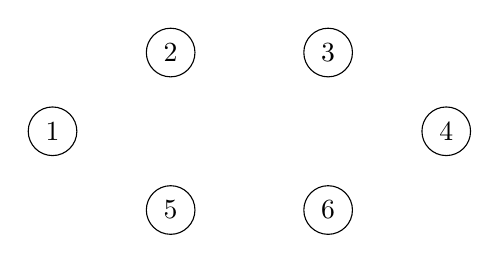
\begin{tikzpicture}
\node[draw, circle] (1) at (1.5,2) {$1$};
\node[draw, circle] (2) at (3,3) {$2$};
\node[draw, circle] (3) at (5,3) {$3$};
\node[draw, circle] (4) at (6.5,2) {$4$};
\node[draw, circle] (5) at (3,1) {$5$};
\node[draw, circle] (6) at (5,1) {$6$};
%\path[draw,thick,-] (1) -- node[font=\small,label=above:3] {} (2);
%\path[draw,thick,-] (2) -- node[font=\small,label=above:5] {} (3);
%\path[draw,thick,-] (3) -- node[font=\small,label=above:9] {} (4);
%\path[draw,thick,-] (1) -- node[font=\small,label=below:5] {} (5);
%\path[draw,thick,-] (5) -- node[font=\small,label=below:2] {} (6);
%\path[draw,thick,-] (6) -- node[font=\small,label=below:7] {} (4);
%\path[draw,thick,-] (2) -- node[font=\small,label=left:6] {} (5);
%\path[draw,thick,-] (3) -- node[font=\small,label=left:3] {} (6);
\end{tikzpicture}
\end{center}
Ensimmäinen virittävään puuhun lisättävä
kaari on 5--6, joka yhdistää
komponentit $\{5\}$ ja $\{6\}$ komponentiksi $\{5,6\}$:
\\
\begin{center}
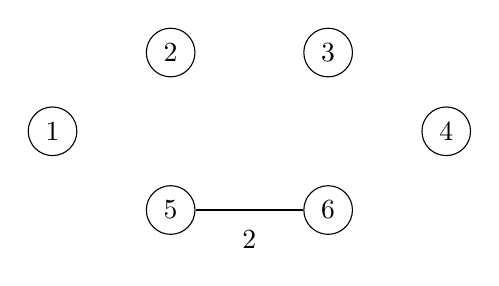
\begin{tikzpicture}
\node[draw, circle] (1) at (1.5,2) {$1$};
\node[draw, circle] (2) at (3,3) {$2$};
\node[draw, circle] (3) at (5,3) {$3$};
\node[draw, circle] (4) at (6.5,2) {$4$};
\node[draw, circle] (5) at (3,1) {$5$};
\node[draw, circle] (6) at (5,1) {$6$};

%\path[draw,thick,-] (1) -- node[font=\small,label=above:3] {} (2);
%\path[draw,thick,-] (2) -- node[font=\small,label=above:5] {} (3);
%\path[draw,thick,-] (3) -- node[font=\small,label=above:9] {} (4);
%\path[draw,thick,-] (1) -- node[font=\small,label=below:5] {} (5);
\path[draw,thick,-] (5) -- node[font=\small,label=below:2] {} (6);
%\path[draw,thick,-] (6) -- node[font=\small,label=below:7] {} (4);
%\path[draw,thick,-] (2) -- node[font=\small,label=left:6] {} (5);
%\path[draw,thick,-] (3) -- node[font=\small,label=left:3] {} (6);
\end{tikzpicture}
\end{center}
Tämän jälkeen algoritmi lisää puuhun vastaavasti
kaaret 1--2, 3--6 ja 1--5:
\\
\begin{center}
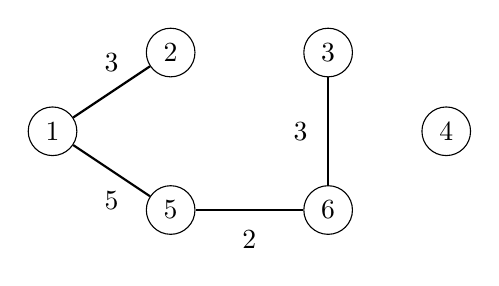
\begin{tikzpicture}
\node[draw, circle] (1) at (1.5,2) {$1$};
\node[draw, circle] (2) at (3,3) {$2$};
\node[draw, circle] (3) at (5,3) {$3$};
\node[draw, circle] (4) at (6.5,2) {$4$};
\node[draw, circle] (5) at (3,1) {$5$};
\node[draw, circle] (6) at (5,1) {$6$};

\path[draw,thick,-] (1) -- node[font=\small,label=above:3] {} (2);
%\path[draw,thick,-] (2) -- node[font=\small,label=above:5] {} (3);
%\path[draw,thick,-] (3) -- node[font=\small,label=above:9] {} (4);
\path[draw,thick,-] (1) -- node[font=\small,label=below:5] {} (5);
\path[draw,thick,-] (5) -- node[font=\small,label=below:2] {} (6);
%\path[draw,thick,-] (6) -- node[font=\small,label=below:7] {} (4);
%\path[draw,thick,-] (2) -- node[font=\small,label=left:6] {} (5);
\path[draw,thick,-] (3) -- node[font=\small,label=left:3] {} (6);
\end{tikzpicture}
\end{center}

Näiden lisäysten jälkeen monet
komponentit ovat yhdistyneet ja verkossa on kaksi
komponenttia: $\{1,2,3,5,6\}$ ja $\{4\}$.

Seuraavaksi käsiteltävä kaari on 2--3,
mutta tämä kaari ei tule mukaan puuhun,
koska solmut 2 ja 3 ovat jo samassa komponentissa.
Vastaavasta syystä myöskään kaari 2--5 ei tule mukaan puuhun.

Lopuksi puuhun tulee kaari 4--6,
joka luo yhden komponentin:
\\
\begin{center}
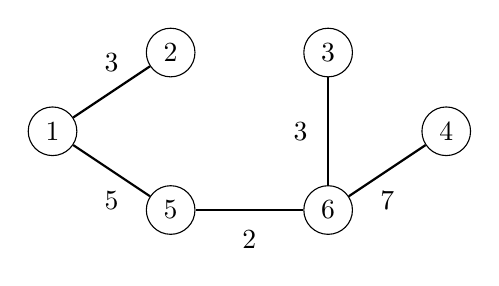
\begin{tikzpicture}
\node[draw, circle] (1) at (1.5,2) {$1$};
\node[draw, circle] (2) at (3,3) {$2$};
\node[draw, circle] (3) at (5,3) {$3$};
\node[draw, circle] (4) at (6.5,2) {$4$};
\node[draw, circle] (5) at (3,1) {$5$};
\node[draw, circle] (6) at (5,1) {$6$};

\path[draw,thick,-] (1) -- node[font=\small,label=above:3] {} (2);
%\path[draw,thick,-] (2) -- node[font=\small,label=above:5] {} (3);
%\path[draw,thick,-] (3) -- node[font=\small,label=above:9] {} (4);
\path[draw,thick,-] (1) -- node[font=\small,label=below:5] {} (5);
\path[draw,thick,-] (5) -- node[font=\small,label=below:2] {} (6);
\path[draw,thick,-] (6) -- node[font=\small,label=below:7] {} (4);
%\path[draw,thick,-] (2) -- node[font=\small,label=left:6] {} (5);
\path[draw,thick,-] (3) -- node[font=\small,label=left:3] {} (6);
\end{tikzpicture}
\end{center}

Tuloksena on verkon pienin virittävä puu,
jonka paino on $2+3+3+5+7=21$.

Kruskalin algoritmin
tuloksena on aina pienin mahdollinen
virittävä puu.
Tämä johtuu siitä, että
kahden komponentin
yhdistämisessä mahdollisimman kevyt kaari
on aina paras valinta,
koska muuten komponentit täytyisi yhdistää
myöhemmin käyttäen raskaampaa kaarta.

\subsubsection{Toteutus}

Seuraava koodi on runko Kruskalin algoritmin
toteutukselle.
Koodi olettaa, että verkon kaaret on tallennettu kaarilistana
niin, että taulukot \texttt{a} ja \texttt{b}
kertovat kaaren alku- ja loppusolmun
ja taulukko \texttt{w} kertoo kaaren painon.
Kaarilistan tulee olla järjestyksessä
kaarten painojen mukaisesti.

Koodi käyttää kahta funktiota:
funktio \texttt{sama} tutkii,
ovatko solmut samassa komponentissa,
ja funktio \texttt{liita}
yhdistää kaksi komponenttia toisiinsa.

\begin{lstlisting}
int c = 0; // virittävän puun koko
for (int i = 1; i <= m; i++) {
    if (sama(a[i],b[i])) continue;
    liita(a[i],b[i]);
    c += w[i];
}
\end{lstlisting}

Ongelmana on, kuinka toteuttaa tehokkaasti
funktiot \texttt{sama} ja \texttt{liita}.
Seuraavaksi esiteltävä tietorakenne
ratkaisee asian.
Se toteuttaa kummankin funktion
ajassa $O(\log n)$,
jolloin Kruskalin algoritmin
aikavaativuus on $O(m \log n)$
kaarilistan järjestämisen jälkeen.

\section{Union-find-rakenne}

Union-find-rakenne pitää yllä
alkiojoukkoja.
Joukot ovat erillisiä,
eli tietty alkio on tarkalleen
yhdessä joukossa.
Rakenne tarjoaa kaksi operaatiota,
jotka toimivat ajassa $O(\log n)$.
Ensimmäinen operaatio tarkistaa,
ovatko kaksi alkiota samassa joukossa.
Toinen operaatio yhdistää kaksi
joukkoa toisiinsa.

\subsubsection{Rakenne}

Union-find-rakenteessa jokaisella
joukolla on edustaja-alkio.
Kaikki muut joukon alkiot osoittavat
edustajaan joko suoraan tai
muiden alkioiden kautta.

Esimerkiksi jos joukot ovat
$\{1,4,7\}$, $\{5\}$ ja $\{2,3,6,8\}$,
tilanne voisi olla:
\\
\begin{center}
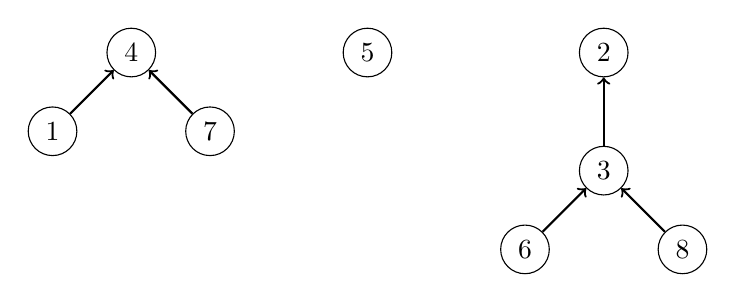
\begin{tikzpicture}
\node[draw, circle] (1) at (0,-1) {$1$};
\node[draw, circle] (2) at (7,0) {$2$};
\node[draw, circle] (3) at (7,-1.5) {$3$};
\node[draw, circle] (4) at (1,0) {$4$};
\node[draw, circle] (5) at (4,0) {$5$};
\node[draw, circle] (6) at (6,-2.5) {$6$};
\node[draw, circle] (7) at (2,-1) {$7$};
\node[draw, circle] (8) at (8,-2.5) {$8$};

\path[draw,thick,->] (1) -- (4);
\path[draw,thick,->] (7) -- (4);

\path[draw,thick,->] (3) -- (2);
\path[draw,thick,->] (6) -- (3);
\path[draw,thick,->] (8) -- (3);

\end{tikzpicture}
\end{center}
~\\
Tässä tapauksessa alkiot 4, 5 ja 2
ovat joukkojen edustajat.

Minkä tahansa alkion edustaja
löytyy kulkemalla polku loppuun alkiosta.
Esimerkiksi alkion 6 edustaja on 2,
koska polku on $6 \rightarrow 3 \rightarrow 2$.
Tämän avulla voi selvittää,
ovatko kaksi alkiota samassa joukossa:
jos kummankin alkion edustaja on sama,
alkiot ovat samassa joukossa,
ja muuten eri joukoissa.

Joukkojen yhdistäminen tapahtuu
valitsemalla toisen edustaja
joukkojen yhteiseksi edustajaksi
ja kytkemällä toinen edustaja siihen.
Esimerkiksi joukot $\{1,4,7\}$ ja $\{2,3,6,8\}$
voi yhdistää näin joukoksi $\{1,2,3,4,6,7,8\}$:
\\
\begin{center}
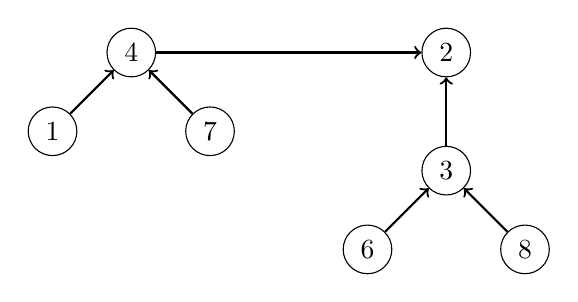
\begin{tikzpicture}
\node[draw, circle] (1) at (2,-1) {$1$};
\node[draw, circle] (2) at (7,0) {$2$};
\node[draw, circle] (3) at (7,-1.5) {$3$};
\node[draw, circle] (4) at (3,0) {$4$};
\node[draw, circle] (6) at (6,-2.5) {$6$};
\node[draw, circle] (7) at (4,-1) {$7$};
\node[draw, circle] (8) at (8,-2.5) {$8$};

\path[draw,thick,->] (1) -- (4);
\path[draw,thick,->] (7) -- (4);

\path[draw,thick,->] (3) -- (2);
\path[draw,thick,->] (6) -- (3);
\path[draw,thick,->] (8) -- (3);

\path[draw,thick,->] (4) -- (2);
\end{tikzpicture}
\end{center}
~\\
Tästä lähtien alkio 2 edustaa kaikkia joukon alkioita.

Tehokkuuden kannalta oleellista on,
miten yhdistäminen tapahtuu.
Osoittautuu, että ratkaisu on yksinkertainen:
riittää yhdistää aina pienempi joukko suurempaan,
tai kummin päin tahansa,
jos joukot ovat yhtä suuret.

Tätä menetelmää käyttäen pisin mahdollinen ketju
alkiosta edustajaan on aina luokkaa $O(\log n)$,
eli operaatiot ovat tehokkaita.

\subsubsection{Toteutus}

Union-find-rakenne on kätevää toteuttaa
taulukoiden avulla.
Seuraavassa toteutuksessa taulukko \texttt{k}
viittaa seuraavaan alkioon ketjussa
tai alkioon itseensä, jos alkio on edustaja.
Taulukko \texttt{s} taas kertoo jokaiselle edustajalle,
kuinka monta alkiota niiden joukossa on.

\newpage
Aluksi jokainen alkio on omassa joukossaan,
jonka koko on 1:

\begin{lstlisting}
for (int i = 1; i <= n; i++) k[i] = i;
for (int i = 1; i <= n; i++) s[i] = 1;
\end{lstlisting}

Funktio \texttt{sama} kertoo,
ovatko alkiot samassa joukossa:

\begin{lstlisting}
bool sama(int a, int b) {
    while (a != k[a]) a = k[a];
    while (b != k[b]) b = k[b];
    return a == b;
}
\end{lstlisting}

Funktio \texttt{liita} taas yhdistää
kaksi joukkoa toisiinsa:

\begin{lstlisting}
void liita(int a, int b) {
    while (a != k[a]) a = k[a];
    while (b != k[b]) b = k[b];
    if (s[a] > s[b]) {
        s[a] += s[b];
        k[b] = a;
    } else {
        s[b] += s[a];
        k[a] = b;
    }
}
\end{lstlisting}

\section{Primin algoritmi}

Primin algoritmi on vaihtoehtoinen menetelmä
verkon pienimmän virittävän puun muodostamiseen.
Algoritmi aloittaa puun muodostamisen valitusta
verkon solmusta ja lisää puuhun aina kaaren,
joka on mahdollisimman kevyt ja joka
liittää puuhun uuden solmun.

\subsubsection{Toiminta}

Tarkastellaan Primin algoritmin toimintaa
seuraavassa verkossa:
\\
\begin{center}
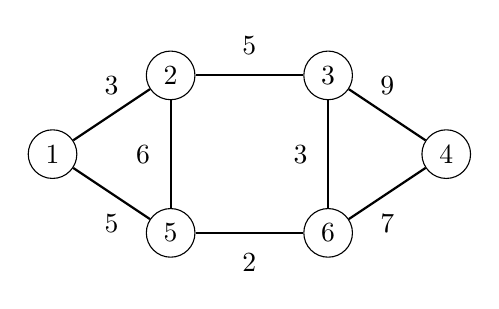
\begin{tikzpicture}
\node[draw, circle] (1) at (1.5,2) {$1$};
\node[draw, circle] (2) at (3,3) {$2$};
\node[draw, circle] (3) at (5,3) {$3$};
\node[draw, circle] (4) at (6.5,2) {$4$};
\node[draw, circle] (5) at (3,1) {$5$};
\node[draw, circle] (6) at (5,1) {$6$};
\path[draw,thick,-] (1) -- node[font=\small,label=above:3] {} (2);
\path[draw,thick,-] (2) -- node[font=\small,label=above:5] {} (3);
\path[draw,thick,-] (3) -- node[font=\small,label=above:9] {} (4);
\path[draw,thick,-] (1) -- node[font=\small,label=below:5] {} (5);
\path[draw,thick,-] (5) -- node[font=\small,label=below:2] {} (6);
\path[draw,thick,-] (6) -- node[font=\small,label=below:7] {} (4);
\path[draw,thick,-] (2) -- node[font=\small,label=left:6] {} (5);
\path[draw,thick,-] (3) -- node[font=\small,label=left:3] {} (6);

%\path[draw=red,thick,-,line width=2pt] (5) -- (6);
\end{tikzpicture}
\end{center}

\newpage
Aluksi solmujen välillä ei ole mitään kaaria:
\begin{center}
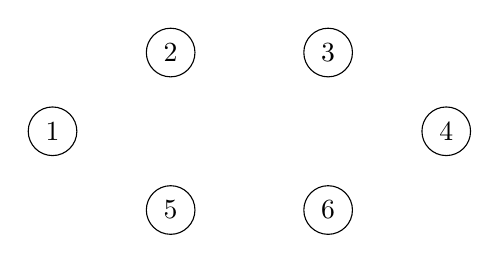
\begin{tikzpicture}
\node[draw, circle] (1) at (1.5,2) {$1$};
\node[draw, circle] (2) at (3,3) {$2$};
\node[draw, circle] (3) at (5,3) {$3$};
\node[draw, circle] (4) at (6.5,2) {$4$};
\node[draw, circle] (5) at (3,1) {$5$};
\node[draw, circle] (6) at (5,1) {$6$};
%\path[draw,thick,-] (1) -- node[font=\small,label=above:3] {} (2);
%\path[draw,thick,-] (2) -- node[font=\small,label=above:5] {} (3);
%\path[draw,thick,-] (3) -- node[font=\small,label=above:9] {} (4);
%\path[draw,thick,-] (1) -- node[font=\small,label=below:5] {} (5);
%\path[draw,thick,-] (5) -- node[font=\small,label=below:2] {} (6);
%\path[draw,thick,-] (6) -- node[font=\small,label=below:7] {} (4);
%\path[draw,thick,-] (2) -- node[font=\small,label=left:6] {} (5);
%\path[draw,thick,-] (3) -- node[font=\small,label=left:3] {} (6);
\end{tikzpicture}
\end{center}

Puun muodostuksen voi aloittaa mistä tahansa solmusta,
ja aloitetaan se nyt solmusta 1.
Kevein kaari on painoltaan 3 ja se johtaa solmuun 2:
\begin{center}
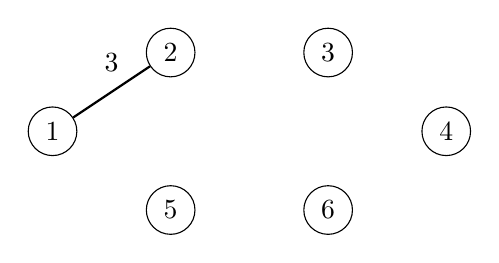
\begin{tikzpicture}
\node[draw, circle] (1) at (1.5,2) {$1$};
\node[draw, circle] (2) at (3,3) {$2$};
\node[draw, circle] (3) at (5,3) {$3$};
\node[draw, circle] (4) at (6.5,2) {$4$};
\node[draw, circle] (5) at (3,1) {$5$};
\node[draw, circle] (6) at (5,1) {$6$};
\path[draw,thick,-] (1) -- node[font=\small,label=above:3] {} (2);
%\path[draw,thick,-] (2) -- node[font=\small,label=above:5] {} (3);
%\path[draw,thick,-] (3) -- node[font=\small,label=above:9] {} (4);
%\path[draw,thick,-] (1) -- node[font=\small,label=below:5] {} (5);
%\path[draw,thick,-] (5) -- node[font=\small,label=below:2] {} (6);
%\path[draw,thick,-] (6) -- node[font=\small,label=below:7] {} (4);
%\path[draw,thick,-] (2) -- node[font=\small,label=left:6] {} (5);
%\path[draw,thick,-] (3) -- node[font=\small,label=left:3] {} (6);
\end{tikzpicture}
\end{center}

Nyt kevein uuteen solmuun johtavan
kaaren paino on 5,
ja voimme laajentaa joko solmuun 3 tai 5.
Valitaan solmu 3:
\begin{center}
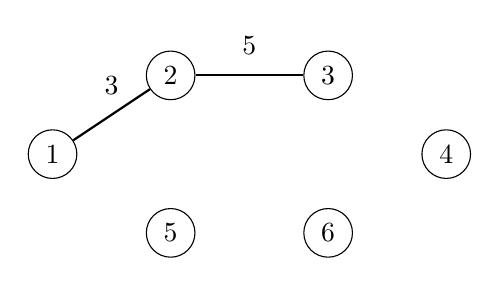
\begin{tikzpicture}
\node[draw, circle] (1) at (1.5,2) {$1$};
\node[draw, circle] (2) at (3,3) {$2$};
\node[draw, circle] (3) at (5,3) {$3$};
\node[draw, circle] (4) at (6.5,2) {$4$};
\node[draw, circle] (5) at (3,1) {$5$};
\node[draw, circle] (6) at (5,1) {$6$};
\path[draw,thick,-] (1) -- node[font=\small,label=above:3] {} (2);
\path[draw,thick,-] (2) -- node[font=\small,label=above:5] {} (3);
%\path[draw,thick,-] (3) -- node[font=\small,label=above:9] {} (4);
%\path[draw,thick,-] (1) -- node[font=\small,label=below:5] {} (5);
%\path[draw,thick,-] (5) -- node[font=\small,label=below:2] {} (6);
%\path[draw,thick,-] (6) -- node[font=\small,label=below:7] {} (4);
%\path[draw,thick,-] (2) -- node[font=\small,label=left:6] {} (5);
%\path[draw,thick,-] (3) -- node[font=\small,label=left:3] {} (6);
\end{tikzpicture}
\end{center}
Sama jatkuu, kunnes kaikki solmut ovat mukana puussa:
\begin{center}
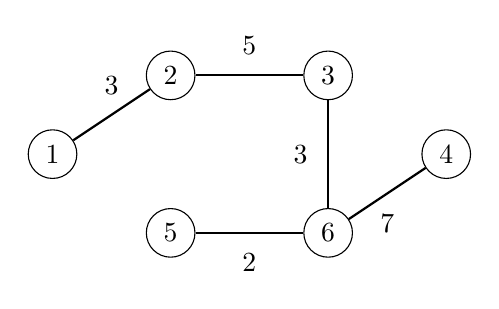
\begin{tikzpicture}
\node[draw, circle] (1) at (1.5,2) {$1$};
\node[draw, circle] (2) at (3,3) {$2$};
\node[draw, circle] (3) at (5,3) {$3$};
\node[draw, circle] (4) at (6.5,2) {$4$};
\node[draw, circle] (5) at (3,1) {$5$};
\node[draw, circle] (6) at (5,1) {$6$};
\path[draw,thick,-] (1) -- node[font=\small,label=above:3] {} (2);
\path[draw,thick,-] (2) -- node[font=\small,label=above:5] {} (3);
%\path[draw,thick,-] (3) -- node[font=\small,label=above:9] {} (4);
%\path[draw,thick,-] (1) -- node[font=\small,label=below:5] {} (5);
\path[draw,thick,-] (5) -- node[font=\small,label=below:2] {} (6);
\path[draw,thick,-] (6) -- node[font=\small,label=below:7] {} (4);
%\path[draw,thick,-] (2) -- node[font=\small,label=left:6] {} (5);
\path[draw,thick,-] (3) -- node[font=\small,label=left:3] {} (6);
\end{tikzpicture}
\end{center}

\subsubsection{Toteutus}

Primin algoritmi muistuttaa Dijkstran algoritmia,
ja sen voi toteuttaa samaan tapaan prioriteettijonolla.
Erona on, että Dijkstran algoritmissa valitaan kaari,
jonka kautta syntyy lyhin polku alkusolmusta uuteen solmuun,
mutta Primin algoritmissa valitaan vain kevein kaari,
joka johtaa uuteen solmuun.

Algoritmin aikavaativuus on $O(n + m \log m)$
eli sama kuin Dijkstran algoritmissa.
Käytännössä Primin algoritmi on suunnilleen
yhtä nopea kuin Kruskalin algoritmi,
eli on makuasia, kumpaa algoritmia käyttää.

